\documentclass[12pt]{article}

\usepackage{hyperref} %links in ToC
\usepackage{caption} %interesting things with captions
\usepackage[margin=1.5in]{geometry} %mostly set margin of the report
\usepackage{tabulary} %text wrapping in tables
\usepackage{subcaption} %let me put multiple images into a single caption
\usepackage{textcomp} %let me use \textrangle{} to get '>'

%images being embeded
\usepackage{graphicx}
\graphicspath{ {images/} }

%code highlighting
\usepackage{minted}
\setminted[c++]{frame=single,linenos=true,autogobble=true,numbersep=4pt,tabsize=4}
\setminted[bash]{frame=single,linenos=true,autogobble=true,numbersep=4pt,tabsize=4}
\setminted[xml]{frame=single,linenos=true,autogobble=true,numbersep=4pt,tabsize=4}

%fix a quote mark issue
\usepackage [english]{babel}
\usepackage [autostyle, english = american]{csquotes}
\MakeOuterQuote{"}


\begin{document}
\pagenumbering{gobble}
\begin{titlepage}
	\centering
	{\Huge Virtualisation\par}
	\vspace{0.25in}
	{\Large Project 1\par}
	\vspace{2in}
	{Alex Harper\par}
	\newpage
\end{titlepage}
\pagenumbering{roman}
\tableofcontents
\newpage

\listoffigures
% \listoftables
\newpage
\setlength{\parindent}{4em} %indent of first line of paragraph
\setlength{\parskip}{1em} %space between paragraphs

\pagenumbering{arabic}

% \section{topics}
% \begin{verbatim}

% ---ADDING TESTS TO GLOP CONFIG---
% if i need to pad more pages, but i want to try not haing to do this
% \end{verbatim}

\section{Introduction}

This project has been my first time using Visual Studio and git on Windows.
While I do not really like either things, they do work if you use them correctly.
In this paper I go over what I did to get ready for working with Windows for programming as well as some specific programming bits.

The programming I show here is mostly for me to play with Visual Studio to work out what quirks it has.
I took that opportunity to get Goole Test setup in a project and do some basic tests, which was a bit of a learning curve for me.
For the tests, I was pushing how far I could get bad code to still work correctly by doing obviously wrong things.
I also give some basic code examples of making classes, because that is what the book goes over.

\section{Visual Studio}

Since I am always the odd man out by using linux, I have to cave and meet the enviroment that my group partners are going to be using.
This means Windows and Visual Studio.
I have touched Visual Studio before in the form of the reskined Atmel Studio to do micro controller programming, but that was fairly different than the original.

Installing the IDE was simple with downloading the installer and running it.
It gave some options and I made sure to get the C++ compiler installed.

\begin{figure}[ht]
	\centering
	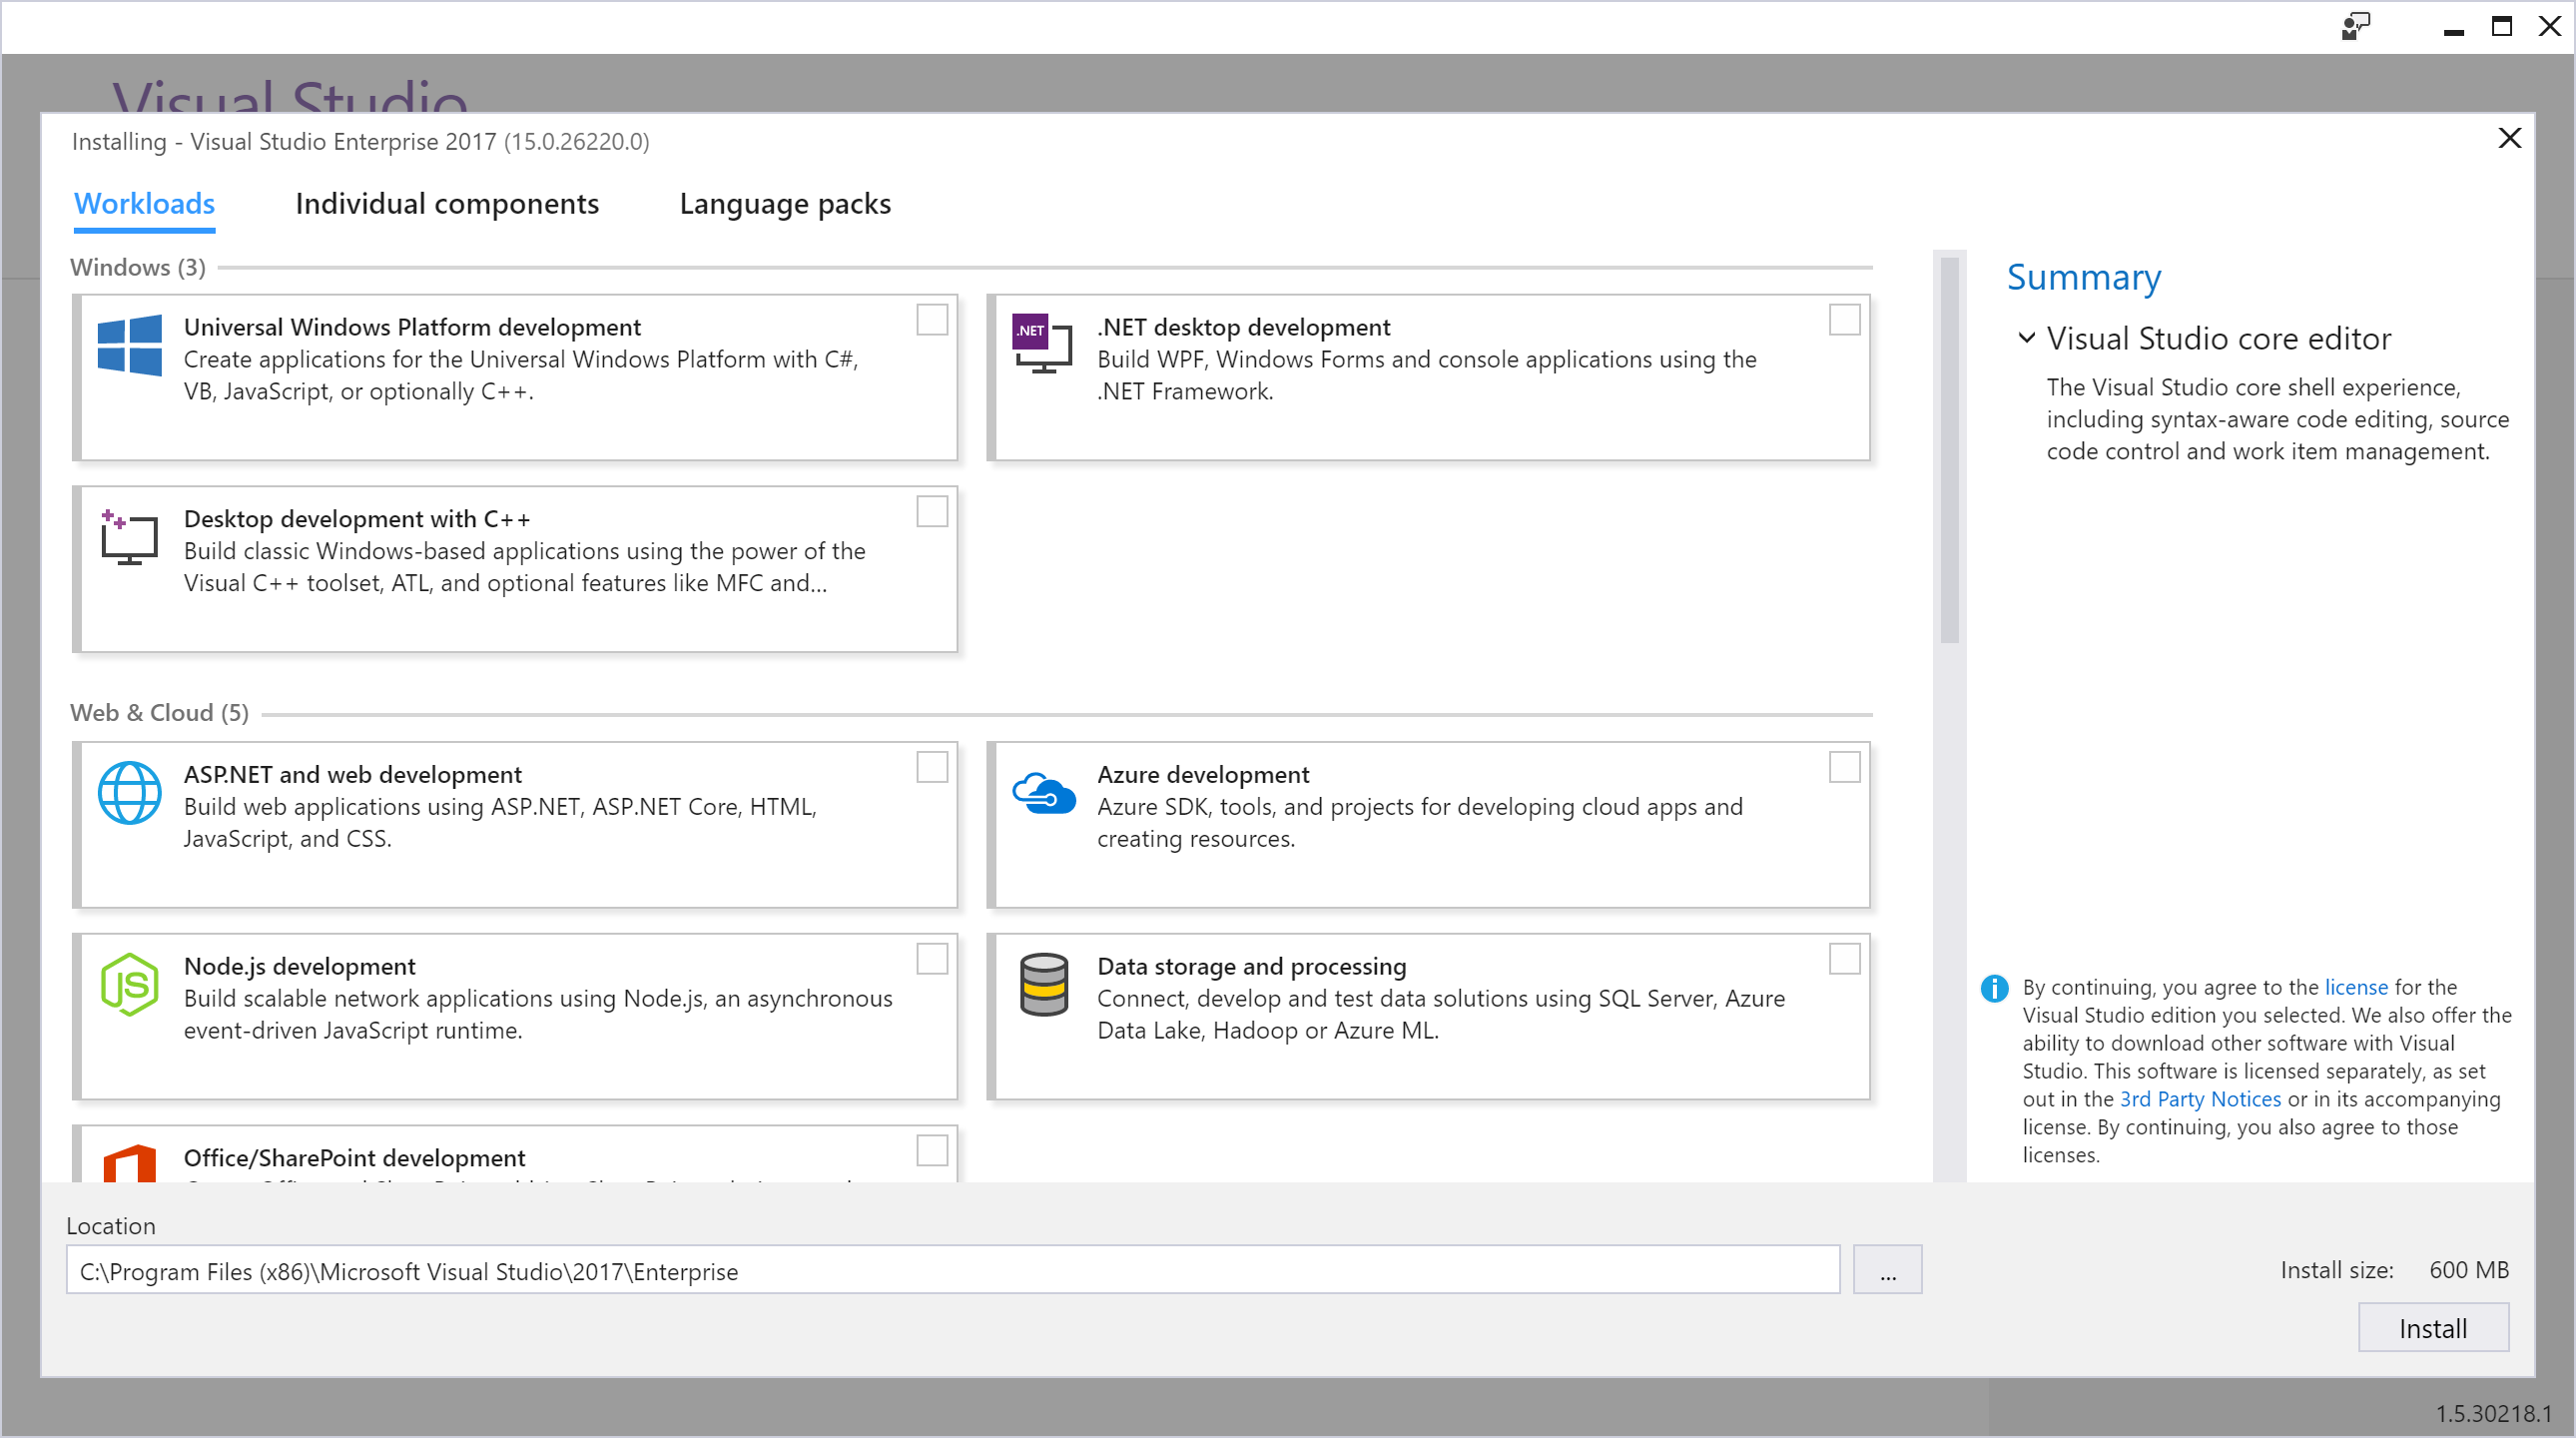
\includegraphics[width=\textwidth]{vs_installer.png}
	\caption{Window of Installer to Select extra Components}
	\label{fig:vs_installer}
\end{figure}

After getting installed, it was time to mess around with it and see what it is like.
I made a new "solution" and made sure the compiler worked, and that things operated for the basics.
It is fairly similar to what I have used before, just different keyboard bindings.

After messing around a few minutes, I made a list of things I don't like about the program, but in general are not very major.
\begin{itemize}
	\item Missing Features that I am used to having
	\begin{itemize}
		\item When the variable is a pointer to an object, pressing the '.' button does not automatically translate it into '-$>$'
		\item The suggestions pane while typing does not automaticly come back when I accidentally dismiss it (but ctrl+space brings it up)
		\item The suggestions pane while typing does not select the first entry in the box  by default and waits for me to press the down button. This messes me up a lot with my muscle memory
		\item The block comment shortcuts are stupid. It should be a toggle of commenting the block and not make the person have to remember two different buttons.
		\item The "toggle header/source file" shortcuts don't even work
	\end{itemize}
	\item When asking it to build or start a test, it takes a second or two to even start the process. There is no reason it should take that long
	\item It broke on me once, simply not building. A simple restart of the program fixed it, but why did it decide to stop working?
	\item There seems to be no way to select a location in a repository to put a solution made in visual studio, making me have to externally manage it. Not a huge deal
\end{itemize}

\section{Google Test}

For the testing framework, our group has decided to use Google Test.
It is a simple framework that lets you simply define a group of code and explicitly set test conditions.
The framework handles running the tests and trys to gracefully handle any exceptions in the tests (and marks those as failures).
To install the framework, it was simple with the built in tool that manages extra plugin stuff for Visual Studio.
In the start menu search for "visual studio installer" and then click the buttons shown in fig\ref{fig:modify_button} and fig\ref{fig:google_test_plugin}.

\begin{figure}[ht]
	\centering
	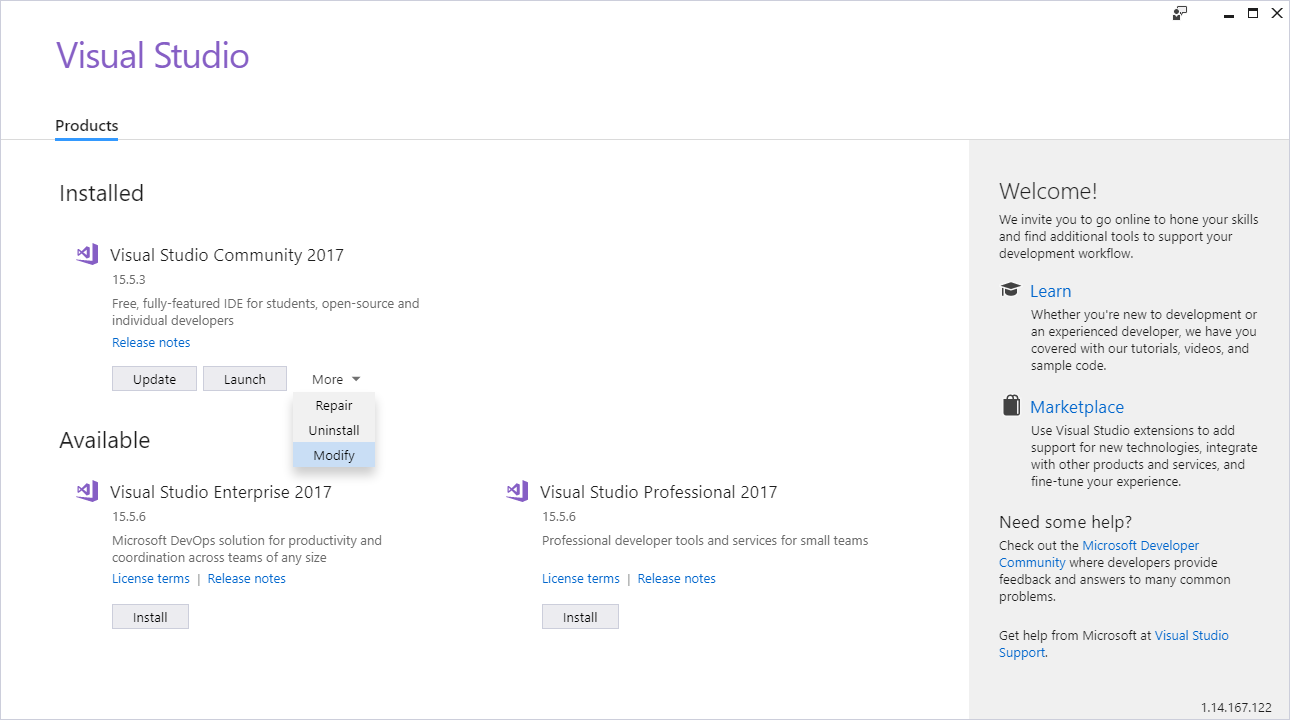
\includegraphics[width=\textwidth]{modify_button.png}
	\caption{Button To Press In The "Installer" To Add Components To Visual Studio}
	\label{fig:modify_button}
\end{figure}

\begin{figure}[ht]
	\centering
	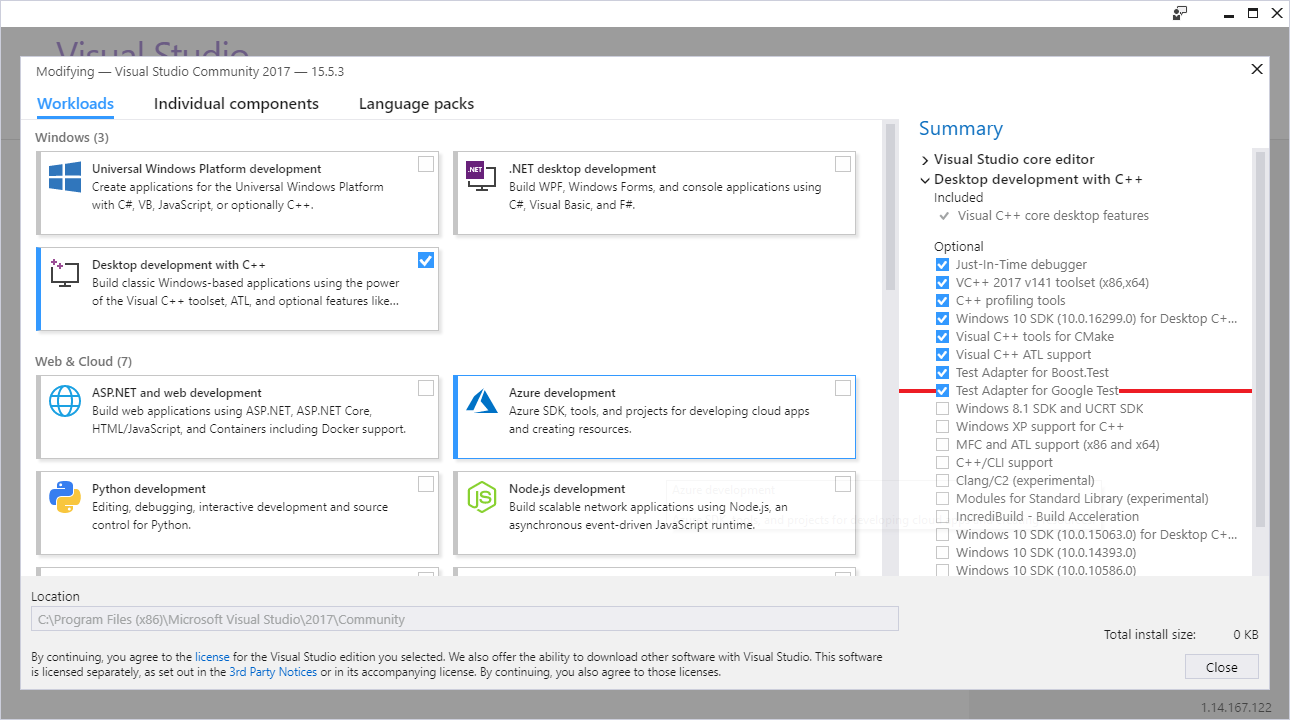
\includegraphics[width=\textwidth]{google_test_plugin.png}
	\caption{Checkbox Location For Google Test - Highlighted In Red}
	\label{fig:google_test_plugin}
\end{figure}

After getting it installed, it is time to make a new project to use google test.
This is where I got confused and spen about an hour going in circles.
Visual Studio has two different things of a "solution" and a "project".
Only a single solution can be open at a time, but it can contain several projects.
I had thought that they were the same thing and as I went to make a new project, instead I made a new solution.
When you go to "File - New - Project" it defaults to making a new solution at the same time and not putting it in the current solution which already had my code in it.
There is a dropbox for making it add to the current solution, but instead I will continue to opt for what is fig\ref{fig:vs_new_project}.

\begin{figure}[ht]
	\centering
	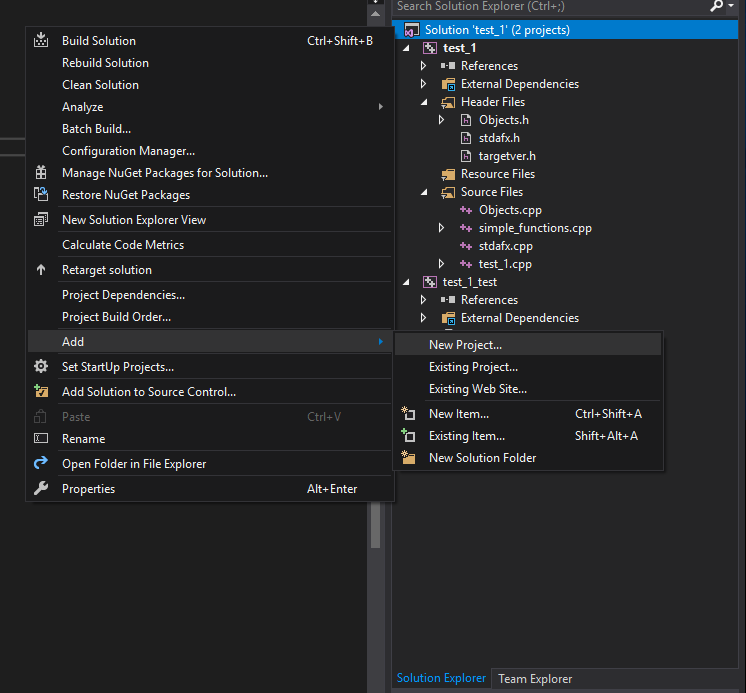
\includegraphics[width=0.6\textwidth]{vs_new_project.png}
	\caption{How I Will Add Projects To My Current Solution From Now On}
	\label{fig:vs_new_project}
\end{figure}

And now that the framework is installed, lets make some tests.
At first I decided to only do super basics, but it devolved into a short exploration of abusing the memory layout of objects and see what technically works and didn't break things.
In fig\ref{fig:example_test} is an example test case that shows the very basic usage.
In fig\ref{fig:test_explorer} shows the test explorer pane in visual studio.

\begin{figure}[ht]
	\centering
	\begin{minted}{c++}
		TEST(TestGroupName, TestName) {
			EXPECT_EQ(1, 1);
			EXPECT_TRUE(true);
		}
	\end{minted}
	\vspace{-15pt}
	\caption{Example Test Case Using Google Test}
	\label{fig:example_test}
\end{figure}

\begin{figure}[!ht]
	\centering
	\begin{subfigure}[t]{0.45\textwidth}
		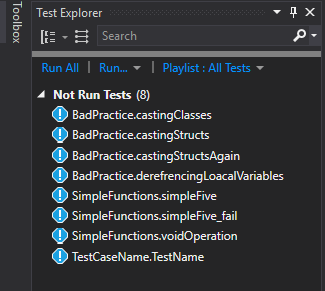
\includegraphics[width=\textwidth]{not_run_tests.png}
		\caption{Tests Before Running Them}
	\end{subfigure}
	\begin{subfigure}[t]{0.45\textwidth}
		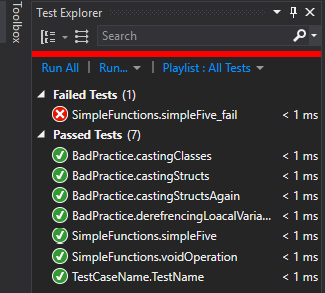
\includegraphics[width=\textwidth]{run_tests.png}
		\caption{Tests After Running Them}
	\end{subfigure}
	\begin{subfigure}[t]{0.45\textwidth}
		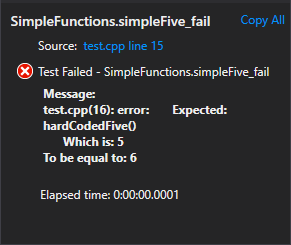
\includegraphics[width=\textwidth]{failed_test_summary.png}
		\caption{Summary of a Failed Test}
	\end{subfigure}
	\caption{Test Explorer Pane In Visual Studio}
	\label{fig:test_explorer}
\end{figure}

\clearpage
\section{Git on Windows}

This is where things took a large departure from what I was expecting.
I am very familure using git with a command line and I like the simplicity of it.
The extension in visual studio is something that I am not used to, as it feels opaque to me.
Really the operation of it is simple and the same as normal git, but I still like my command line.
In fig\ref{fig:team_explorer} is a picture of what the add-on looks like.

\begin{figure}[!ht]
	\centering
	\begin{subfigure}[t]{0.45\textwidth}
		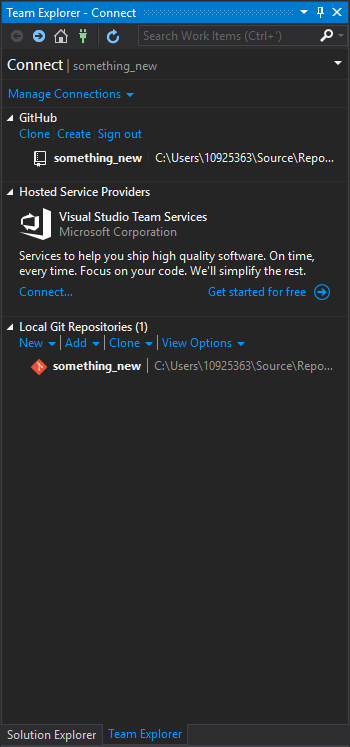
\includegraphics[width=\textwidth]{team_explorer.png}
		\caption{Team Explorer With Github}
	\end{subfigure}
	\begin{subfigure}[t]{0.45\textwidth}
		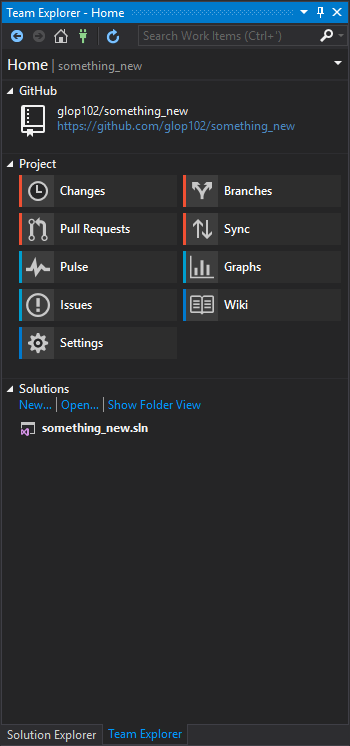
\includegraphics[width=\textwidth]{github_repo.png}
		\caption{Local Repo with Various Buttons}
		\label{fig:repo_buttons}
	\end{subfigure}
	\caption{Team Explorer Pane In Visual Studio}
	\label{fig:team_explorer}
\end{figure}

The team explorer pane is a builtin part of the program already, but is limited to only working with microsoft services.
The github extension adds the extra field of letting github be the back end that code is stored on.
As you can see in fig\ref{fig:repo_buttons}, it has quick access buttons for the typical actions.
The "changes" button is where you make commits to the current branch.
The "sync" button is where you push or pull code.
The "branches" button is where you do merges and such.

After messing with it, I suggest starting by making the new repo with github first.
Place the repo where you want before making the new "solution" in VS.
When you make the new "solution", change the location to the repo folder that was just made.
Now when you go to the changes button with the plugin, it will let you add a commit message and push the files up.
Note: When you make the repo, make sure to have a .gitignore file get made to keep all the trash that visual studio puts in from making your repo get huge in size.

While this seems kindof handy, I still prefer using the command line directly.
I am used to a workflow on the command line under linux.
The idea of an IDE is neat, but I typically only use it for a handy text editor that gives suggestions as I type.
It will be an interesting experiance as I work with my team on this.

\section{Screwing With Classes}

As the section fo the book is about how to make classes with various restrictions and features, I suppose I should mention some things about that myself.
I simply added this code into my test project for Google Test.

The book has many pages about specifics of what to do for exact situations.
I instead am just going to give a short list of things here that sumarize the important bits.

\begin{figure}[ht]
	\begin{minted}{c++}
	\end{minted}
	\caption{Simple Subclass}
	\label{fig:class_ex1}
\end{figure}

\end{document}